\chapter{جمع‌بندی، نتیجه‌گیری و پیشنهادات}


\section{جمع‌بندی و نتیجه‌گیری}
در این پروژه سعی بر این شد که سیستمی برای نگهداری و تشخیص خرابی گره‌های موجود در یک شبکه‌ی اشیاء بر اساس \cite{jung2017vibration} توسعه یابد. هدف این سیستم پیش‌بینی زمان خرابی دستگاه‌های مختلف بر اساس تحلیل نحوه‌ی لرزش موتور آنها بود.

ابتدا در فصل ۲ تمام تکنولوژی‌ها و ابزارهایی که برای پیاده‌سازی این سیستم از آنها استفاده‌شده است را عنوان کردیم و همه‌ی آنها را با جزئیات توضیح دادیم.

در فصل ۳ انواع روش‌های موجود برای استقرار مدل یادگیری ماشین و استفاده از آن شرح داده‌شدند و بنابر نیازمندی‌های پروژه و ماهیت استفاده از مدل یادگیری ماشین برای مسئله‌ی پیش‌بینی میزان عمر مفید باقی‌مانده، استقرار بی‌درنگ را انتخاب کردیم.

در فصل ۴ نیز نحوه‌ی توسعه و معماری کارگزاری که برای دریافت درخواست‌های کاربران و همچنین ارسال پاسخ‌های تحلیل‌های سیستم پیاده شده‌ بود را شرح دادیم. سپس در فصل ۵ نحوه‌ی توسعه‌ی مدل یادگیری ماشین بر اساس ویژگی‌های بدست‌آمده از داده‌های خام لرزش گره‌های موجود در شبکه‌ی اشیاء توضیح داده‌شد. درنهایت یک مدل خطی برای پیش‌بینی میزان عمر مفید باقی‌مانده بر اساس مقدار متفاوت‌بودن آن دستگاه نسبت به یک دستگاه سالم پیشنهاد داده‌شد.


در مراحل مختلف این پروژه نیز چالش‌ها و محدودیت‌های بر سر راهمان قرار گرفتند که در این قسمت به تعدادی از آنها اشاره می‌کنیم: 

\begin{itemize}

\item انتخاب روش استقرار مناسب برای مدل یادگیری ماشین: همانطور که در فصل سوم توضیح دادیم، روش‌های مختلفی برای استقرار مدل‌های یادگیری ماشین وجود دارند که بنا به انتخاب هر کدام، نحوه‌ی شروع یادگیری، نحوه‌ی ذخیره‌ و ارسال نتایج پیش‌بینی و روش بروزرسانی مدل یادگیری ماشین متفاوت است. این مورد باید حتما پیش از شروع توسعه‌ی مدل یادگیری ماشین مشخص می‌شد تا برای مواردی که بیان شد، بهترین روش را برگزینیم.

\item انتخاب پارامتر‌های مناسب: نحوه‌ی هموار کردن و استفاده از پارامترهای مناسب پنجره‌ی هان نیز یکی از موارد چالش‌برانگیز دیگر بود. این پارامترها باید با توجه به تعداد نمونه‌های موجود در یک اندازه‌گیری طوری  انتخاب شود که سیگنال خیلی هموار نشود به نحوی که ویژگی ذاتی خود را از دست بدهد. با انتخاب حالت‌های مختلف، مناسب‌ترین گزینه انتخاب شد.

\item نبود مجموعه داده‌ی مناسب: یکی از بزرگ‌ترین محدودیت‌ها در طی انجام این پروژه نبود مجموعه‌ی داده‌‌ی مناسب و برچسب‌دار برای استفاده‌ی مدل یادگیری ماشین بود. از آنجا که مسئله‌ی پیش بینی عمر مفید باقی‌مانده‌ی هر دستگاه، هم یک مسئله‌ی طبقه‌بندی (باید کلاس کاری دستگاه مشخص شود) و هم یک مسئله‌ی رگرسیون (عمر باقی‌مانده‌ی دستگاه باید مشخص شود) می‌باشد، نیازمند دو مجموعه داده‌ی کامل برچسب‌دار بودیم که فراهم نشد. یکی از مهم‌ترین دلایلی که مجموعه داده‌ی آماده برای این نوع مسئله در دسترس عموم قرار ندارد این است که اکثر پروژه‌هایی که در این باب انجام شده‌اند صنعتی بوده و رویکرد هر کدام و نحوه‌ی طبقه‌بندی و پارامترهای دخیل (لرزش، دما، رطوبت، صدا، ارتفاع از سطح دریا) در تحلیل داده برای هر کدام متفاوت است.

\end{itemize}


\section{پیشنهادات}

پروژه‌ی کنونی قابلیت توسعه و افزایش کارایی را در بخش‌های مختلفی اعم از میکروسرویس‌های توسعه‌ی یافته برای کارگزار اصلی، مدل هوش مصنوعی هم از لحاظ عملکرد و هم از لحاظ سرعت و همچنین اضافه کردن قابلیت تشخیص نوع خرابی را داراست. در بخش‌های زیر پیشنهاداتی را برای کارهای آینده و مرتبط با این پروژه آورده‌ایم.

\subsubsection{پیاده‌کردن سیستم ارسال گزارش و هشدار به مدیران}
با افزایش تعداد گره‌های موجود در سیستم، کار نظارت درست بر این گره‌ها برای مدیران سخت می‌شود. از طرفی ارائه‌ی گزارشی دقیق از عملکرد دستگاه‌های مختلف هم به مدیران و هم به سازندگان قطعات می‌تواند مفید باشد. همچنین پیاده‌سازی بخشی برای ارسال هشدار به مدیران جهت اطلاع دادن از خرابی قریب‌الوقوع یک دستگاه می‌تواند مدیر را در پیش‌بینی تدابیر مناسب کمک کند.

\subsubsection{تشخیص نوع خرابی}
یکی دیگر از جنبه‌های نگهداری که می‌تواند سود بسیار زیادی را برای صنعت‌گران داشته باشد، تشخیص نوع خرابی در کنار پیش‌بینی زمان خرابی دستگاه‌ها است. سیستمی موسوم به دکتر ماشین‌ها در \cite{patel2020doctor} پیاده شده است که بسته به سیستم‌های مختلف پارامتر‌های مختلفی را در نظر می‌گیرد و در یادگیری مدل بر اساس ویژگی‌های دستگاه‌ها، وزن پارامتر‌ها برای هر کدام از دستگاه‌ها فرق می‌کند. پیاده‌سازی چنین سیستمی قاعدتا نیازمند قدرت پردازشی بسیار بالا در کنار مجموعه داده‌های دقیق و مورد تایید متخصصان است. نمونه‌ای از نحوه‌ی طبقه‌بندی چنین سیستمی در \cref{fig:dom}\cite{patel2020doctor}آورده شده است.

\begin{figure}[!h]
\centerline{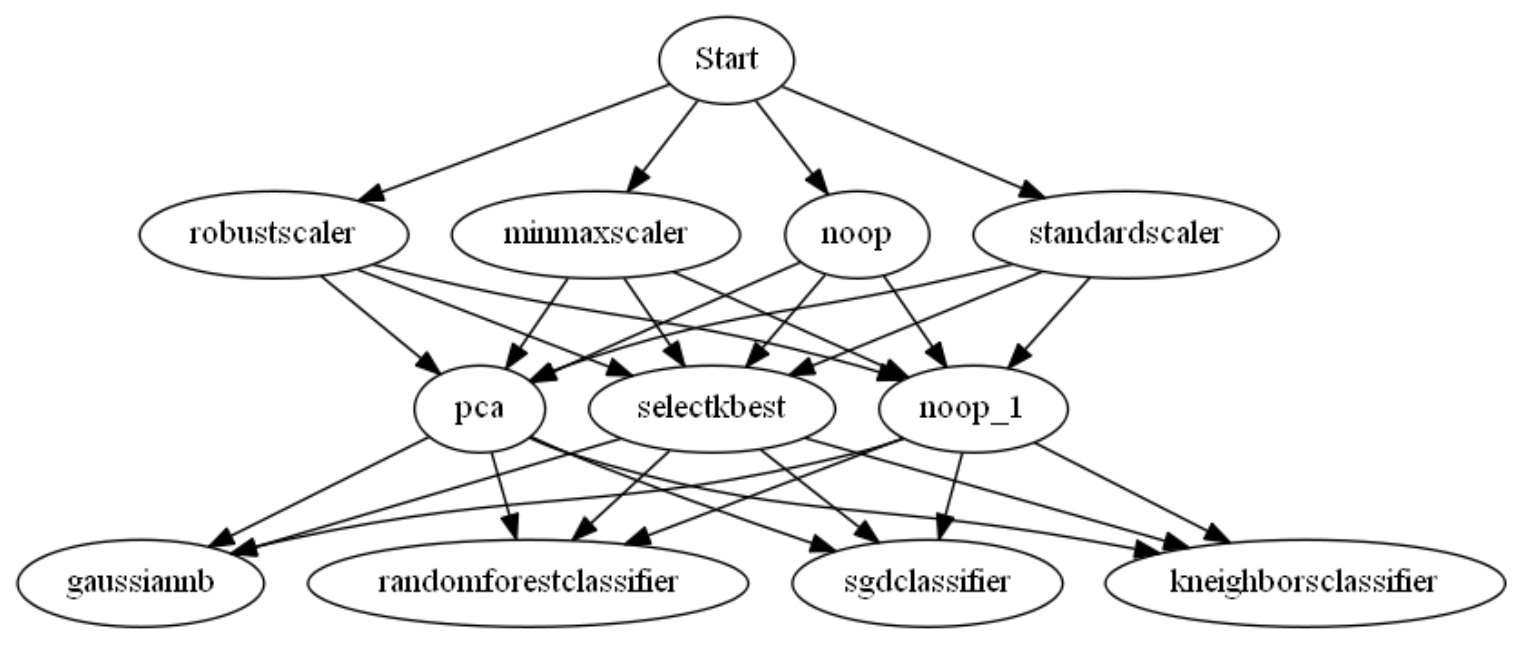
\includegraphics[width=\textwidth]{dom.png}}
\caption{نحوه‌ی طبقه‌بندی مدل یادگیری ماشین بر اساس پارامتر‌های مختلف\cite{patel2020doctor}}
\label{fig:dom}
\end{figure}


\subsubsection{افزایش دقت پیش‌بینی}
رویکردی که در این پروژه از آن استفاده شد تنها لرزش موتور سیستم را در سه بعد در نظر می‌گیرد. یکی از بهبودهایی که می‌توان برای نتایج پیش‌بینی در این پروژه متصور شد، در نظر گرفتن پارامترهای دیگری اعم از دما، شرکت سازنده و رطوبت در کنار لرزش است تا دقت پیش‌بینی‌ها برای میزان عمر مفید باقی‌مانده افزایش یابد. 
